\begin{frame}{トリガー \& DAQ 効率 { \bf (Run68) チャージトリガー }}
  \label{page:trig_Run68}
  \tminipageTwo{
    \small
    $Eff_{DAQ}, Eff_{N trig}$はラン毎に評価\\
    $Eff_{trig}$は$Eff_{K \otimes CDH1}\times Eff_{Charge}$で評価
  }{
    \begin{figure}
      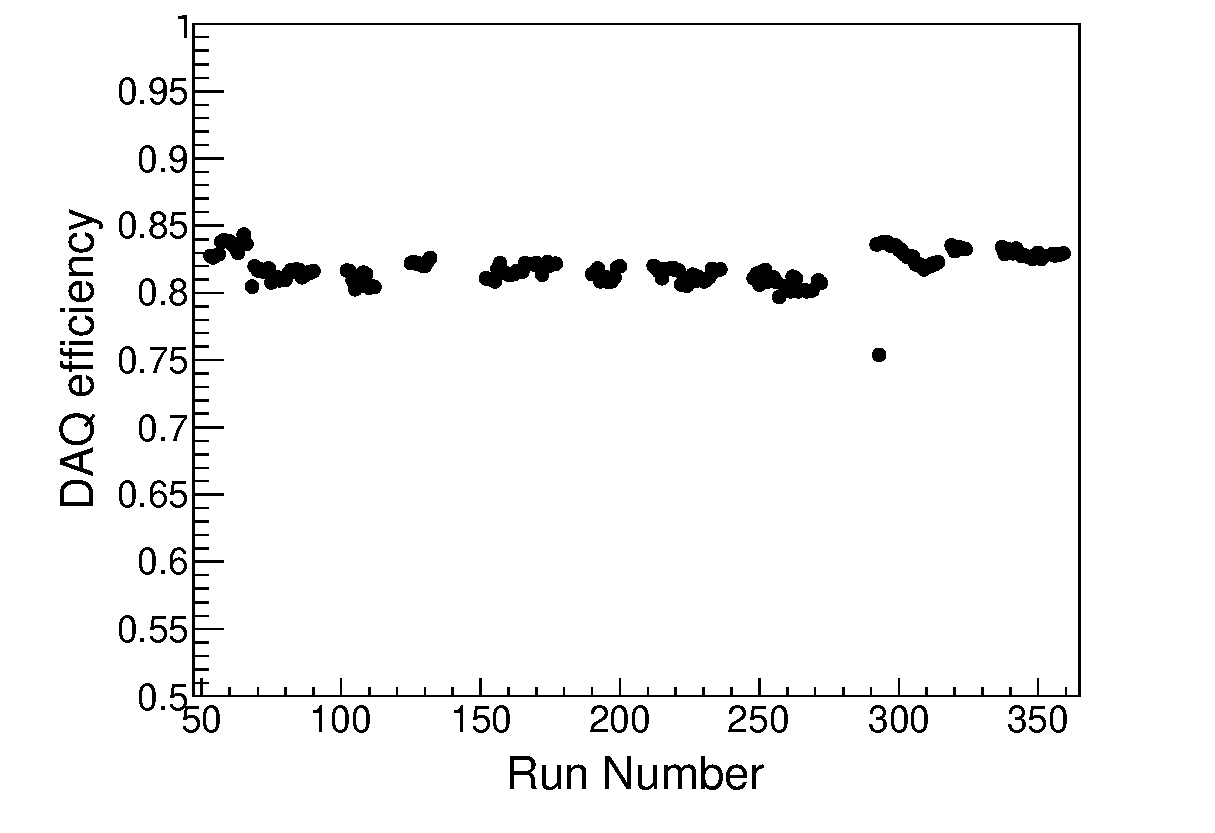
\includegraphics[width=4cm]{../pic/Run68/trigger/DAQ.eps}
    \end{figure}
    \centering    
  }

  \tminipageTwo{
    \begin{figure}
      $K\otimes CDH1$\\
      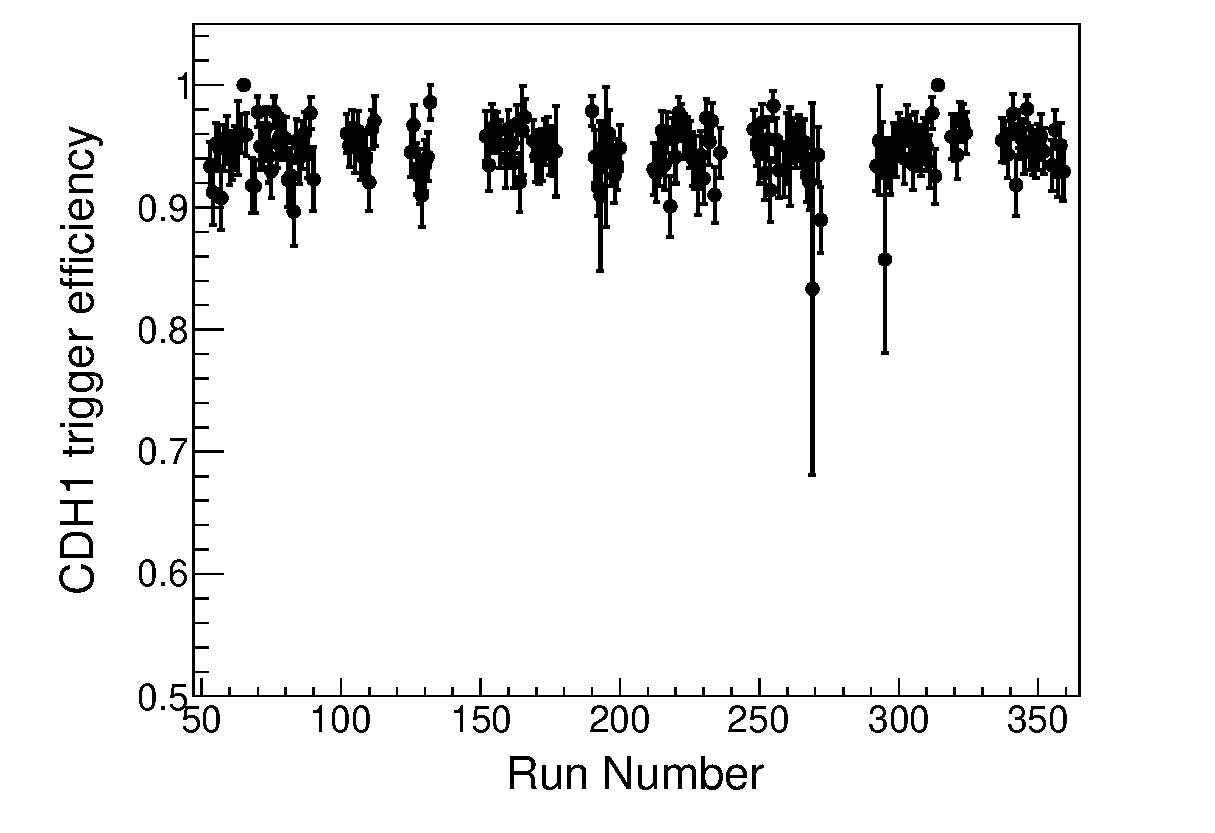
\includegraphics[width=4cm]{../pic/Run68/trigger/CDH1.eps}      
    \end{figure}
    \vspace{-4mm}
    \centering
    \tiny
    バイアスのないKaonトリガーを母数にする
  }{
    \begin{figure}
      $Charge$\\
      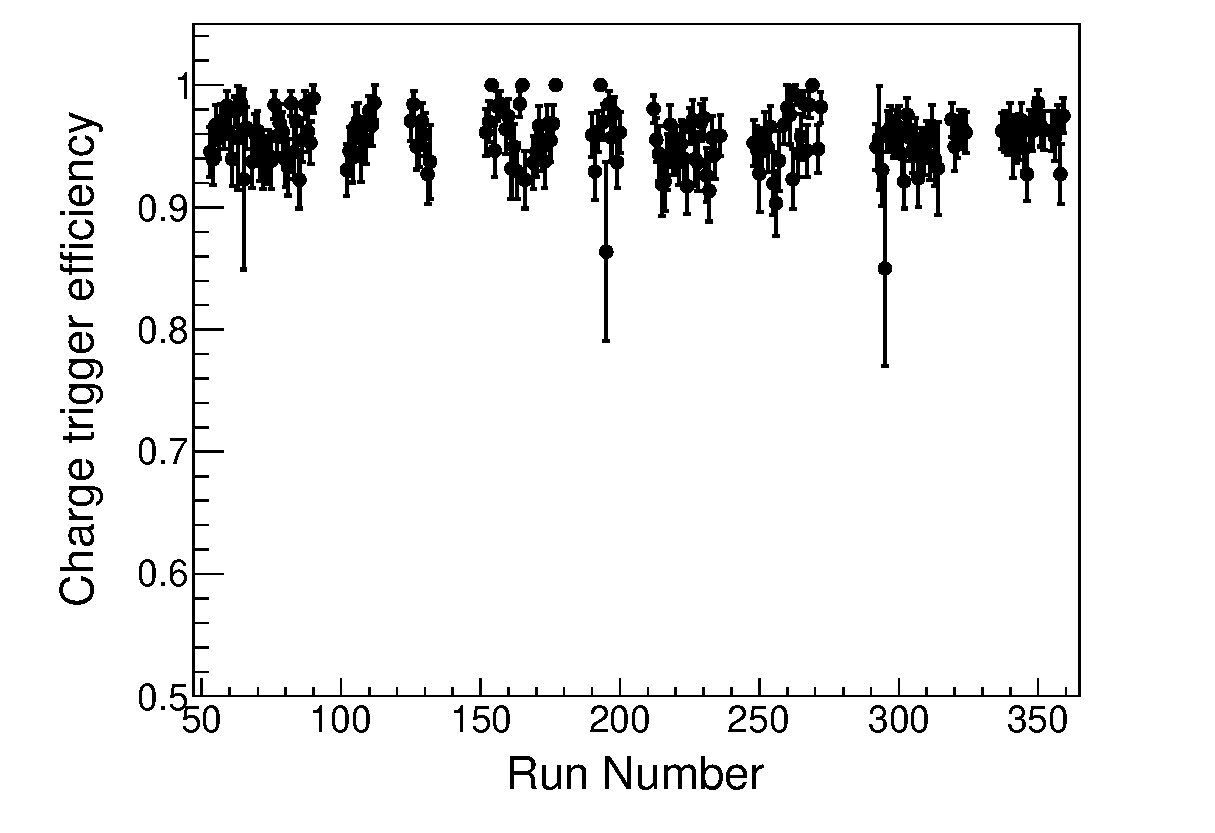
\includegraphics[width=4cm]{../pic/Run68/trigger/Charge.eps}
    \end{figure}
    \vspace{-4mm}
    \centering
    \tiny
    バイアスのない$K \otimes CDH1$トリガーを母数にする
  }

  
\end{frame}
